% THIS DOCUMENT IS TAILORED TO REQUIREMENTS FOR SCIENTIFIC COMPUTING.  IT SHOULDN'T
% BE USED FOR NON-SCIENTIFIC COMPUTING PROJECTS
\documentclass[12pt]{article}

\usepackage{amsmath, mathtools}
\usepackage{amsfonts}
\usepackage{amssymb}
\usepackage{graphicx}
\usepackage{colortbl}
\usepackage{xr}
\usepackage{hyperref}
\usepackage{longtable}
\usepackage{xfrac}
\usepackage{tabularx}
\usepackage{float}
\usepackage{siunitx}
\usepackage{booktabs}
\usepackage{caption}
\usepackage{pdflscape}
\usepackage{afterpage}
\usepackage{enumitem}

\usepackage[round]{natbib}

%\usepackage{refcheck}

\hypersetup{
    bookmarks=true,         % show bookmarks bar?
      colorlinks=true,       % false: boxed links; true: colored links
    linkcolor=red,          % color of internal links (change box color with linkbordercolor)
    citecolor=green,        % color of links to bibliography
    filecolor=magenta,      % color of file links
    urlcolor=cyan           % color of external links
}

%% Comments

\usepackage{color}

\newif\ifcomments\commentstrue %displays comments
%\newif\ifcomments\commentsfalse %so that comments do not display

\ifcomments
\newcommand{\authornote}[3]{\textcolor{#1}{[#3 ---#2]}}
\newcommand{\todo}[1]{\textcolor{red}{[TODO: #1]}}
\else
\newcommand{\authornote}[3]{}
\newcommand{\todo}[1]{}
\fi

\newcommand{\wss}[1]{\authornote{blue}{SS}{#1}} 
\newcommand{\plt}[1]{\authornote{magenta}{TPLT}{#1}} %For explanation of the template
\newcommand{\an}[1]{\authornote{cyan}{Author}{#1}}

%% Common Parts

\newcommand{\progname}{ProgName} % PUT YOUR PROGRAM NAME HERE
\newcommand{\authname}{Team \#, Team Name
\\ Student 1 name
\\ Student 2 name
\\ Student 3 name
\\ Student 4 name} % AUTHOR NAMES                  

\usepackage{hyperref}
    \hypersetup{colorlinks=true, linkcolor=blue, citecolor=blue, filecolor=blue,
                urlcolor=blue, unicode=false}
    \urlstyle{same}
                                


% For easy change of table widths
\newcommand{\colZwidth}{1.0\textwidth}
\newcommand{\colAwidth}{0.13\textwidth}
\newcommand{\colBwidth}{0.82\textwidth}
\newcommand{\colCwidth}{0.1\textwidth}
\newcommand{\colDwidth}{0.05\textwidth}
\newcommand{\colEwidth}{0.8\textwidth}
\newcommand{\colFwidth}{0.17\textwidth}
\newcommand{\colGwidth}{0.5\textwidth}
\newcommand{\colHwidth}{0.28\textwidth}

% Used so that cross-references have a meaningful prefix
\newcounter{defnum} %Definition Number
\newcommand{\dthedefnum}{GD\thedefnum}
\newcommand{\dref}[1]{GD\ref{#1}}
\newcounter{datadefnum} %Datadefinition Number
\newcommand{\ddthedatadefnum}{DD\thedatadefnum}
\newcommand{\ddref}[1]{DD\ref{#1}}
\newcounter{theorynum} %Theory Number
\newcommand{\tthetheorynum}{TM\thetheorynum}
\newcommand{\tref}[1]{TM\ref{#1}}
\newcounter{tablenum} %Table Number
\newcommand{\tbthetablenum}{TB\thetablenum}
\newcommand{\tbref}[1]{TB\ref{#1}}
\newcounter{assumpnum} %Assumption Number
\newcommand{\atheassumpnum}{A\theassumpnum}
\newcommand{\aref}[1]{A\ref{#1}}
\newcounter{constraintnum} %Constraint Number
\newcommand{\rconstraintnum}{C\constraintnum}
\newcommand{\Cref}[1]{C\ref{#1}}
\newcounter{goalnum} %Goal Number
\newcommand{\gthegoalnum}{GS\thegoalnum}
\newcommand{\gsref}[1]{GS\ref{#1}}
\newcounter{instnum} %Instance Number
\newcommand{\itheinstnum}{IM\theinstnum}
\newcommand{\iref}[1]{IM\ref{#1}}
\newcounter{reqnum} %Requirement Number
\newcommand{\rthereqnum}{R\thereqnum}
\newcommand{\rref}[1]{R\ref{#1}}
\newcounter{frnum} %FR Number
\newcommand{\rthefrnum}{FR\thefrnum} 
\newcommand{\frref}[1]{FR\ref{#1}}
\newcounter{nfrnum} %NFR Number
\newcommand{\rthenfrnum}{NFR\thenfrnum}
\newcommand{\nfrref}[1]{NFR\ref{#1}}

\newcounter{lcnum} %Likely change number
\newcommand{\lthelcnum}{LC\thelcnum}
\newcommand{\lcref}[1]{LC\ref{#1}}

\newcounter{ulcnum} %Unlikely change number
\newcommand{\ltheulcnum}{ULC\theulcnum}
\newcommand{\ulcref}[1]{ULC\ref{#1}}

\usepackage{fullpage}

\newcommand{\deftheory}[9][Not Applicable]
{
\newpage
\noindent \rule{\textwidth}{0.5mm}

\paragraph{RefName: } \textbf{#2} \phantomsection 
\label{#2}

\paragraph{Label:} #3

\noindent \rule{\textwidth}{0.5mm}

\paragraph{Equation:}

#4

\paragraph{Description:}

#5

\paragraph{Notes:}

#6

\paragraph{Source:}

#7

\paragraph{Ref.\ By:}

#8

\paragraph{Preconditions for \hyperref[#2]{#2}:}
\label{#2_precond}

#9

\paragraph{Derivation for \hyperref[#2]{#2}:}
\label{#2_deriv}

#1

\noindent \rule{\textwidth}{0.5mm}

}

\begin{document}

\title{Software Requirements Specification \\ \textit{\progname: Smart Budgeting Expense Tracker}} 
\author{\authname}
\date{\today}
	
\maketitle

~\newpage

\pagenumbering{roman}

\tableofcontents

\listoftables

~\newpage

\section*{Revision History}

\begin{table}[h!]
\centering
\caption{Revision History}
\begin{tabularx}{\textwidth}{p{3cm}p{2cm}X}
\toprule {\bf Date} & {\bf Version} & {\bf Notes}\\
\midrule
10/07/2024 & 0.01 & Added in the following sections to the SRS: Reference Materials (1), NFRs (5.2), Likely Changes (6), Unlikely Changes (7), Development Plan (9), Auxiliary Constraints (10)\\
10/08/2024 & 0.02 & Added in the following sections to the SRS: Purpose of Document (2.1), Organization of Document (2.4), User Characteristics (3.2)\\
10/09/2024 & 0.03 & Added in the following sections to the SRS: Characteristics of Intended Reader (2.3), Functional Requirements (5.1)\\
10/10/2024 & 0.04 & Added in the following sections to the SRS: System Constraints (3.3), Requirements Rationale (5.3)\\
10/11/2024 & 0.05 & Enumerate requirements, clean up doc, review\\
10/11/2024 & 0.06 & Add traceability matrix for requirements\\
10/11/2024 & 0.07 & Add reflection to SRS\\
03/08/2025 & 0.08 & Link Requirements Elicitation Report\\
03/08/2025 & 0.09 & Move constants to Section 10\\
\bottomrule 
\end{tabularx}
\end{table}

~\\


~\newpage

\section{Reference Material}

This section records information for easy reference.

\subsection{Table of Units}

N/A; units are not used in this SRS.

\subsection{Table of Symbols}

N/A; symbols are not used in this SRS.

\subsection{Abbreviations and Acronyms}

\renewcommand{\arraystretch}{1.2}
\begin{tabular}{l l} 
  \toprule		
  \textbf{symbol} & \textbf{description}\\
  \midrule 
  AI & Artificial Intelligence\\
  CI & Continuous Integration\\
  FR & Functional Requirement\\
  JWT & JSON Web Token\\
  LC & Likely Change\\
  ML & Machine Learning\\
  NFR & Non-Functional Requirement\\
  NLP & Natural Language Processing\\
  OCR & Optical Character Recognition\\
  SRS & Software Requirements Specification\\
  ULC & Unlikely Change\\
  UI & User Interface\\
  \bottomrule
\end{tabular}\\

\subsection{Mathematical Notation}

N/A; mathematical notation is not used in this SRS.

\newpage

\pagenumbering{arabic}

\section{Introduction}


\subsection{Purpose of Document}

The purpose of this SRS document is to describe the functional and
non-functional requirements of the Plutos budgeting application. This document
serves as a formal agreement between stakeholders, including developers, project
managers, and end users, to ensure a shared understanding of the system's
objectives, capabilities, and constraints. \\

\noindent The SRS defines the expectations for the project, detailing the system
features, behaviour, and performance requirements. It serves as a reference
throughout the development lifecycle, guiding the design, implementation,
testing, and validation phases to ensure the final product meets the agreed-upon
specifications. Additionally, this document will support future maintenance and
scalability of the application by providing clear and detailed requirements that
facilitate ongoing enhancements.\\

\noindent The requirements specified in this document are based on the findings
from the requirements elicitation process with end users, as detailed in the
\href{https://github.com/PlutosCapstone/Plutos/tree/main/docs/Extras/RequirementsElicitationReport.pdf}{Requirements
Elicitation Report}.

\subsection{Scope of Requirements} 

The scope of this project encompasses the development of a budgeting application, Plutos, that automates expense tracking 
and categorization using AI. The system is designed to address key pain points for young adults struggling to manage their 
finances, specifically focusing on automating the process of tracking spending through receipt scanning, categorization of 
expenses, providing metrics to users regarding their spending habits, and providing feedback on how users can meet their 
budgeting goals.\\

\noindent However, some features that are outside the scope of the project (though may be implemented later) are: 

\begin{itemize}
  \item The system will not account for complex financial scenarios such as investments, stock portfolios, or retirement planning.
  \item Advanced financial forecasting or predictive analytics beyond simple budgeting trends will not be implemented.
  \item The AI model will not handle non-standard or highly complex receipts (e.g., multi-page invoices or handwritten receipts).
  \item The application will not offer integration with external financial accounts such as credit cards or bank accounts.
  \item The model will be trained to detect receipt data from Fortinos and will not initially support various receipt formats.
\end{itemize}

\noindent These exclusions allow the project to concentrate on core features, such as receipt scanning and expense categorization, while ensuring a manageable scope for the development process.

\subsection{Characteristics of Intended Reader} \label{sec_IntendedReader}
The primary audience for this SRS document is the group of undergraduate
software engineering students who will oversee and complete the project’s design
and implementation. This group of specialists, which includes system architects,
software developers, and quality assurance testers, has extensive experience in
the range of technologies needed for the project. Through their coursework and
personal experiences, they are familiar with the process of developing mobile
applications, and as they move through the project milestones, they will deepen
their understanding of artificial intelligence (AI) and machine learning (ML).
They will actively learn how to apply AI/ML technologies in real-world
circumstances throughout the project, which will advance their development as
software engineers. The collaborative effort will help them improve their
real-world application development abilities as the project progresses through
seven milestones, ensuring that they are prepared to produce a practical and
user-friendly budgeting solution.
\subsection{Organization of Document}

The following sections of the SRS will further describe the system and its requirements. The sections will be as follows:

\begin{enumerate}
	\setcounter{enumi}{2}
	\item General System Description
	\item Specific System Description
	\item Requirements
	\item Likely Changes
	\item Unlikely Changes
	\item Traceability Matrices and Graphs
	\item Development Plan
	\item Values of Auxiliary Constants
\end{enumerate}

\newpage

\section{General System Description}

This section provides general information about the system.  It identifies the
interfaces between the system and its environment, describes the user
characteristics and lists the system constraints.

\subsection{System Context}

\begin{figure}[h!]
  \centering
   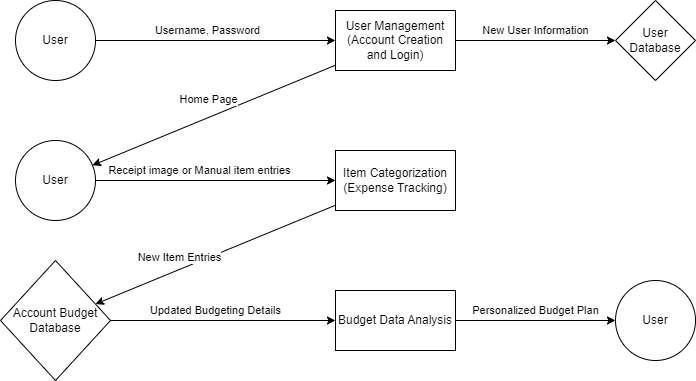
\includegraphics[width=\textwidth]{SystemContext.png}
  \caption{System Context}
  \label{Fig_SystemContext} 
\end{figure}

The system context for this project consists of a user(s), an expense tracking system, 
a budgeting analysis generator, and several databases. The user provides expense 
tracking inputs, such as physical/digital receipts or manual expense entries, and 
receives financial assessments. The expense tracking system processes user inputs, 
generates budgetary evaluations, and interacts with the financial analysis program 
and databases. The expense tracking system is also responsible for ensuring the 
validity of all inputs and provides a response if an invalid input is identified. 
The budgeting analysis generator provides expense categorization and evaluation 
functionalities, such as data analysis and visualization, and supports the expense 
tracking system in generating outputs. The database will be used to store user 
account information, user budget data, and supports the expense tracking system 
in storing and retrieving specific items and their respective categories. 
The system will typically be used for personal finance management, budgeting, 
and expense tracking, and may also be used for educational purposes. While 
the system is not safety-critical, it is important to ensure that the system is 
reliable and accurate in its calculations and analysis to provide users with 
trustworthy insights into their financial situation.

\subsection{User Characteristics} \label{SecUserCharacteristics}

The users of the \textit{Plutos} budgeting application can be grouped into four main categories based on their financial experience and needs. These groups represent varying levels of financial literacy and desired interaction with budgeting tools.

\begin{enumerate}
	\item \textbf{First and Second-Year Undergraduate Students [Primary]} \\ 
		This group consists of young adults who are new to managing their finances independently, such as those living away from home for the first time. The characteristics of these users are as follows:
		\begin{itemize}
			\item \textbf{Financial Knowledge:} Limited experience with budgeting, managing expenses like rent and groceries. Usually have limited financial independence.
			\item \textbf{Time Management:} Busy schedules juggling school, work, and social commitments. Likely to prefer simple, intuitive interfaces that reduce time spent on budgeting.
			\item \textbf{Pain Points:} Lack of education on budgeting, potential to overspend due to unfamiliarity with managing day-to-day expenses.
		\end{itemize}
	\item \textbf{Upper-Year Undergraduate and Post-Graduate Students [Secondary]}
		This group includes more experienced students who have more financial independence as they have had experience managing their finances (in previous years living independently).  They have a better understanding of budgeting and have developed more mature spending habits.
		\begin{itemize}
			\item \textbf{Financial Knowledge:}  Some experience balancing school and work, likely to have a clearer understanding of budgeting needs and differentiating between wants and needs.
			\item \textbf{Time Management:} Likely to have more experience managing limited time and money, though they may still struggle with large financial decisions such as housing or loans.
			\item \textbf{Pain Points:}  May underestimate or overestimate budget needs, particularly with larger expenses.
		\end{itemize}
	\item \textbf{Early Career Professionals [Tertiary]}
		New graduates or individuals recently introduced to the workforce fall into this category. They likely have more stable incomes and financial independence.
		\begin{itemize}
			\item \textbf{Financial Knowledge:} More knowledgeable about saving, budgeting, and managing recurring expenses but still learning to navigate significant financial decisions.
			\item \textbf{Time Management:} May experience stress due to work-related issues and life changes such as moving to a new city and budgeting/tracking expenses may be another stress inducer on top of the new environment.
			\item \textbf{Pain Points:} Struggles with planning for long-term financial goals or managing joint accounts with a partner.
		\end{itemize}
	\item \textbf{Retirees [Tertiary]}
		Although retirees are not a primary focus, they may use the application to simplify financial tracking and planning for a fixed income.
		\begin{itemize}
			\item \textbf{Financial Knowledge:} Likely to have extensive experience with financial management but may struggle to adapt to modern budgeting tools.
			\item \textbf{Time Management:} Older users may face physical limitations (e.g., difficulty typing or navigating) and slower adaptation to new technologies.
			\item \textbf{Pain Points:} Difficulty managing finances without a steady income and adapting to increased living expenses.
		\end{itemize}
\end{enumerate}

\newpage

\subsection{System Constraints}


\begin{enumerate}[label=C\arabic*]
  \item The system must be developed as a mobile application using a
  cross-platform framework (e.g., React Native, Flutter) to ensure
  compatibility with both iOS and Android devices.
  \item The system must utilize a cloud-based backend technology (e.g., AWS,
  Firebase) to provide scalability, reliability, and compatibility across
  environments.
  \item The system must integrate with a third-party OCR library (e.g.,
  Tesseract OCR, Google Vision API) to provide OCR functionality. This is a
  constraint because it is not necessary to reinvent the wheel and build an OCR
  system from scratch.
  \item The system must implement secure password storage and authentication
  mechanisms using a trusted third-party authentication service (e.g., Auth0,
  Firebase). This is to ensure secure user data handling and privacy.
  \item The project must implement a Continuous Integration (CI) pipeline using
  GitHub Actions that automatically runs tests, checks code quality, and
  verifies builds with every commit. This is to ensure that the code is always
  in a deployable state.
  \item The system shall use a dependency management tool (e.g., npm for
  JavaScript, pip for Python) to track external libraries. This is to ensure
  organized dependency management across different working environments. 
\end{enumerate}

\newpage

% ----------------
% SECTION 4
% ----------------
\section{Specific System Description}

This section first presents the problem description, which gives a high-level
view of the problem to be solved. Following this, a solution characteristics
specification is typically included; however this aspect is not applicable for
this SRS.


\subsection{Problem Description}\label{Sec_pd}

The problem description can be found in Section 1 of the
\href{https://github.com/PlutosCapstone/Plutos/blob/main/docs/ProblemStatementAndGoals/ProblemStatement.pdf}{Problem
Statements and Goals} document.

\subsubsection{Terminology and  Definitions}

This subsection provides a list of terms that are used in the subsequent
sections and their meaning, with the purpose of reducing ambiguity and making it
easier to correctly understand the requirements:

\begin{itemize}
  \item \textbf{User Database}: A secure storage location for user information,
  including usernames, passwords, and personal financial profiles.
  \item \textbf{Item Categorization}: The classification of expenses and income
  into distinct categories, such as groceries, rent, and salary, to clarify
  spending habits.
  \item \textbf{Expense Tracking}: The practice of recording and monitoring
  expenditures to understand spending patterns and make informed financial
  decisions.
  \item \textbf{Budget Data Analysis}: The examination of financial data related
  to budgets to identify trends, patterns, and areas for improvement.
  \item \textbf{Personalized Budget Plan}: A customized budget tailored to an
  individual's specific financial goals, income levels, and spending habits.
  \item \textbf{Account Budget Database}: A system for storing and managing
  users' budget data, including allocations, spending limits, and financial
  goals.
  \item \textbf{Digital Financial Tools}: Software applications designed to help
  users manage their finances, including budgeting, tracking expenses, and
  analyzing data.
  \item \textbf{Data Security}: Measures taken to protect personal financial
  information from unauthorized access or breaches.
  \item \textbf{User-Friendly Interface}: An application design that prioritizes
  ease of use and accessibility, making it simple for users to navigate
  financial tools.
\end{itemize}



\subsubsection{Physical System Description} \label{sec_phySystDescrip}

The physical system of \progname{}, includes the following elements: \\

\noindent
\begin{enumerate}[label=PS\arabic*]
  \item[] \textbf{User Interface Elements}
  \item \textbf{Camera Interface}: A feature that enables users to capture
  images of receipts using their mobile device’s camera.
  \item \textbf{Receipt Preview}: A visual display showing the captured
  receipt for user verification before processing.
  \item \textbf{Categorization Display}: An interface that shows identified
  items along with suggested categories for each item.
  \item \textbf{Forms}: Input fields for entering financial data, such as
  income and expenses.
  \item \textbf{Graphs and Charts}: Visual representations of spending
  patterns and budget performance, providing insights into financial health.

  \item[] \textbf{Data Processing Components}
  \item \textbf{Budgeting Algorithm}: An engine that analyzes user data to
  suggest personalized budgets based on historical spending.
  \item \textbf{Notification System}: A feature that alerts users about
  important financial events, such as nearing budget limits.
  \item \textbf{Optical Character Recognition (OCR)}: A technology that
  analyzes the scanned receipt image to extract text, identifying items, prices,
  and totals.
  \item \textbf{Item Categorization Engine}: A module that automatically
  classifies extracted items into predefined categories (e.g., groceries,
  clothing, dining) based on user-defined rules or machine learning algorithms.
  \item \textbf{Database}: A secure storage system for user data, including
  receipts, categorized items, and budget information.
\end{enumerate}

Users interact with the application by entering financial data, setting budgets,
  and reviewing visualizations, using the User Interface Elements (PS1-PS5).
  The system responds by updating financial summaries, processing the
  data, and providing insights based on user behaviour (PS6-PS10).



\subsubsection{Goal Statements}

The goal statements can be found in Section 2 of the
\href{https://github.com/PlutosCapstone/Plutos/blob/main/docs/ProblemStatementAndGoals/ProblemStatement.pdf}{Problem
Statement and Goals} document.

\newpage


\subsection{Solution Characteristics Specification}

\subsubsection{Types}
Not applicable.

\subsubsection{Scope Decisions}
Not applicable.

\subsubsection{Modelling Decisions}
Not applicable.

\subsubsection{Assumptions} \label{sec_assumpt} Not applicable.

\subsubsection{General Definitions}\label{sec_gendef} Not applicable.

\subsubsection{Data Definitions}\label{sec_datadef}

\textbf{Receipt Image Tensor:} \\
The input to the OCR model is a 3D tensor $I \in \mathbb{R}^{H \times W \times C}$ where $H$ is height, $W$ is width, and $C=3$ for RGB channels.\\
\textbf{Detected Item (in receipt): }\\
Each detected item $d_i$ from a receipt is represented as a tuple:
\[
d_i = (n_i, c_i, p_i) \quad \text{where:}
\]
\begin{itemize}
    \item $n_i$ is the item name (string)
    \item $c_i$ is the category (e.g., groceries)
    \item $p_i$ is the price $\in \mathbb{R}^{\geq 0}$
\end{itemize}


\subsubsection{Data Types}\label{sec_datatypes} Not applicable.

\subsubsection{Instance Models} \label{sec_instance}    
Let $\alpha$ be the input image. The OCR model extracts a set of detected characters $T = \{t_1, t_2, \dots, t_n\}$ with corresponding confidence scores $P = \{p_1, p_2, \dots, p_n\}$.\\
Each text element $t_i$ is predicted using a convolutional neural network (CNN) with a softmax layer:
\[
P(t_i \mid \alpha) = \text{softmax}(W f(\alpha) + b)
\]
where $f(\alpha)$ is the image feature vector, $W$ and $b$ are learnable weights and biases.\\
\textbf{Budget Performance Calculation}\\
$BudgetProgress = \frac{TotalSpent}{BudgetLimit} \times 100\%$\\
where $TotalSpent$ is the total amount spent in a category and $BudgetLimit$ is the maximum budget set by the user for the current month.

\subsubsection{Input Data Constraints} \label{sec_DataConstraints}    

Input data constraints are as follows:
\begin{itemize}
  \item Receipt image: $I \in [0, 255]^{H \times W \times 3}$, where $H \leq 2000$, $W \leq 2000$
  \item Max image file size: $S \leq$ \hyperref[Table:AuxConstants]{\textit{MAX\_RECEIPT\_FILE\_SIZE}}
\end{itemize}

\subsubsection{Properties of a Correct Solution} \label{sec_CorrectSolution} Not
applicable.


\newpage


% ----------------
% SECTION 5
% ----------------
\section{Requirements}

This section provides the functional requirements, the business tasks that the
software is expected to complete, and the nonfunctional requirements, the
qualities that the software is expected to exhibit.

The format of each requirement is as follows: `Requirement-ID (Priority Level)
Requierment`. The priority levels are high (H), medium (M), and low (L), and are
used to indicate the importance of the requirement to the system.

\subsection{Functional Requirements}

\textbf{User Account Management Requirements}
\begin{enumerate}[label=FR-UAM-\arabic*]
  \item (H) Users must be able to create an account using a name, email
  address, and password.
  \item (L) Users must be able to update their account information after account
  creation.
  \item (H) Users must be able to log in using their registered email and password.
  \item (H) Users must log in before accessing the application.
  \item (L) Users must be able to log out of their account.
  \item (L) Users must be able to reset their password if forgotten.
\end{enumerate}

\textbf{Receipt Scanning Input Requirements}
\begin{enumerate}[label=FR-IP-\arabic*]
  \item (H) Users must be able to take a picture using the application.
  \item (M) Users must be able to upload an image from their device to the
  application.
  \item (L) The system shall allow a limit of \hyperref[Table:AuxConstants]{\textit{MAX\_RECEIPT\_FILE\_SIZE}} per receipt.
  \item (H) The system must display a preview of the uploaded image, allowing users
  to confirm or retake the image if necessary. 
  \item (H) The system shall upload the confirmed image to the server for processing.
\end{enumerate}

\textbf{Manual Receipt Input Requirements}
\begin{enumerate}[label=FR-MIS-\arabic*]
  \item (M) Users must be able to manually input receipt details. This includes
  items, their associated costs, and the date of purchase.
  \item (M) The system shall validate the input to ensure required fields are
  completed.
  \end{enumerate}

\textbf{Database Management Requirements}
\begin{enumerate}[label=FR-DM-\arabic*]
  \item (H) The system shall store user account information, including usernames,
  email addresses, and passwords, in a secure database.
  \item (H) The system shall store receipt images and extracted data in a secure database.
\end{enumerate}

\textbf{Item Recognition and Categorization Requirements}
\begin{enumerate}[label=FR-RS-\arabic*]
  \item (H) The system shall identify and display item names and costs from the
  uploaded receipt image.
  \item (H) The system shall sort the items into predefined categories, and
  display the category alongside each item.
  \item (H) The user must be able to modify the name, price, and category of the
  identified items.   
\end{enumerate}

\textbf{Financial Tracking Requirements}
\begin{enumerate}[label=FR-FT-\arabic*]
  \item (M) The system shall generate an overview of the user's spending history,
  including total spending by item category and trends over time.
  \item (M) Users shall be able to set up budgets for each spending category.
  \item (M) Users shall be able to view their spending in relation to their set
  budgets.
  \item (L) The system shall notify users when they reach
  \hyperref[Table:AuxConstants]{\textit{NOTIFICATION\_BUDGET\_THRESHOLD}}\%
  of their set budget limit.
  \item (L) The system shall notify users when they achieve specified savings goals.
  \item (L) The system shall store up to 3 years of user transaction history.
\end{enumerate}

\newpage


\subsection{Nonfunctional Requirements}

\textbf{Accuracy Requirements}
\begin{enumerate}[label=NFR-ACC-\arabic*]
  \item (H) The machine learning model must categorize expenses into predefined
  categories (e.g., groceries, utilities, entertainment) with at least
  \hyperref[Table:AuxConstants]{\textit{CATEGORIZATION\_ACCURACY}}\% precision
  to ensure users' financial data is correctly organized.
  \item (H) All monetary calculations (e.g., totals, budgets, currency
  conversions) must maintain a precision of up to
  \hyperref[Table:AuxConstants]{\textit{FINANCIAL\_PRECISION}} decimal places to
  ensure accurate financial reporting.
  \item (H) The OCR model must correctly recognize text from images of receipts
  with a minimum accuracy rate of
  \hyperref[Table:AuxConstants]{\textit{OCR\_ACCURACY}}\%, ensuring minimal
  manual corrections by users.
  \item (H) The application must guarantee
  \hyperref[Table:AuxConstants]{\textit{CALCULATION\_PRECISION}}\% precision in
  summing up expenses, incomes, and savings across different periods and
  categories.
  \item (M) The application should ensure
  \hyperref[Table:AuxConstants]{\textit{SYNC\_CONSISTENCY}}\% consistency of
  financial data upon syncing across multiple devices and sessions.
\end{enumerate}

\textbf{Performance Requirements}
\begin{enumerate}[label=NFR-PERF-\arabic*]
  \item (M) The application must load user account information and financial
  metrics within \hyperref[Table:AuxConstants]{\textit{MAX\_DATA\_LOAD\_TIME}} seconds.
  \item (M) The application must respond to user actions, such as adding a new
  entry or generating a report, by completing the requested operation and
  displaying the result within
  \hyperref[Table:AuxConstants]{\textit{MAX\_INTERACTION\_LOAD\_TIME}} seconds.
  \item (L) The system must be able to handle a minimum of
  \hyperref[Table:AuxConstants]{\textit{MIN\_CONCURRENT\_USERS}} concurrent users
  without significant performance degradation.
\end{enumerate}

\textbf{Usability Requirements}
\begin{enumerate}[label=NFR-USAB-\arabic*]
  \item (M) The application must have a clean, intuitive, and easy-to-navigate
  interface, allowing users to perform common tasks (e.g., adding expenses,
  viewing budgets) within
  \hyperref[Table:AuxConstants]{\textit{MAX\_COMMON\_TASK\_CLICKS}} clicks.
  \item (M) New users should be able to complete the account setup and
  understand core application features within
  \hyperref[Table:AuxConstants]{\textit{MAX\_ACCOUNT\_ONBOARD\_TIME}} minutes.
  \item (L) The application shall provide users with an introductory tutorial and
  tooltips during their first use.
  \item (M) The application shall display error messages within
  \hyperref[Table:AuxConstants]{\textit{MAX\_ERROR\_MESSAGE\_DELAY}} second of
  invalid input submission.
  \item (M) All error messages will include the error type, the invalid 
  input, and a suggested corrective action.
  \item (L) Users should be able to recover from errors (e.g., wrong data entry)
  with no more than
  \hyperref[Table:AuxConstants]{\textit{MAX\_ERROR\_RECOVERY\_STEPS}} steps.
  \item (M) Common user tasks, such as adding a new receipt or setting a budget
  limit, should be completable within
  \hyperref[Table:AuxConstants]{\textit{AVG\_USER\_TASK\_TIME}} seconds on
  average, assuming all required information is readily available.
  \item (M) Information displayed to users shall be concise and relevant, with
  the main dashboard limited to no more than
  \hyperref[Table:AuxConstants]{\textit{MAX\_DISPLAYED\_KEY\_FINANCIAL\_POINTS}}
  key financial data points and advanced options accessible within
  \hyperref[Table:AuxConstants]{\textit{MAX\_ADVANCED\_OPTIONS\_CLICKS}} clicks or less.
  \item (M) User comprehension of the displayed information must exceed\\
  \hyperref[Table:AuxConstants]{\textit{MIN\_USER\_COMPREHENSION}}\%.
\end{enumerate}

\textbf{Security Requirements}
\begin{enumerate}[label=NFR-SEC-\arabic*]
  \item (H) The system must implement secure password storage and authentication
  mechanisms.
  \item (H) The system must ensure that all data transmitted between the client and
  server is encrypted.
\end{enumerate}

\textbf{Maintainability Requirements}
\begin{enumerate}[label=NFR-MTB-\arabic*]
  \item (M) New releases must maintain backward compatibility with previous
  versions, ensuring that users can seamlessly update the application without
  experiencing disruptions in their data or workflows.
  \item (M) Dependencies must be regularly updated (i.e., within major patches)
  to prevent security vulnerabilities and maintain compatibility with new
  features.
  \item (H) At least
  \hyperref[Table:AuxConstants]{\textit{MIN\_CODE\_COVERAGE}}\% of the codebase
  must be covered by automated unit tests to ensure maintainability and minimize
  the risk of introducing bugs when making changes.
\end{enumerate}

\textbf{Portability Requirements}
\begin{enumerate}[label=NFR-PORT-\arabic*]
  \item (H) The software shall be compatible with Android and iOS mobile devices
  running the latest software.
  \item (H) All data must be stored in platform-independent formats (e.g., JSON,
  CSV) for easy transfer and compatibility between devices, databases, and
  systems.
  \item (M) Any external APIs or third-party services integrated into the
  application must support cross-platform usage, ensuring the application can
  access necessary services from any supported platform.
  \item (L) The system must be able to operate in a variety of network
  environments, including Wi-Fi, cellular networks, and offline mode.
\end{enumerate}

\textbf{Reusability Requirements} 
\begin{enumerate}[label=NFR-REUS-\arabic*]
  \item (M) The application must be developed using reusable components (e.g.,
  UI components, API services) where applicable, to prevent code duplication and
  allow for better code maintainability.
  \item (M) The application must adhere to the principle of separation of
  concerns where possible, ensuring that business logic, data access, and
  presentation layers are kept separate and allowing individual layers to be
  reused independently.
  \item (M) Common functionalities (e.g., receipt parsing, authentication, data
  validation) must be abstracted into reusable libraries or modules that can be
  shared across multiple applications or systems.
  \item (L) Design elements (e.g., icons, typography, color schemes) shall be
  created as reusable assets, ensuring they can be reused consistently across
  multiple projects or platforms.
\end{enumerate}

\textbf{Understandability Requirements} 
\begin{enumerate}[label=NFR-UND-\arabic*]
  \item (H) All source code must be thoroughly documented using inline comments
  and external documentation (e.g., README files, docstrings) to ensure that
  developers can easily understand the purpose and behavior of code components.
  \item (H) Variables, functions, classes, and modules must follow consistent
  and meaningful naming conventions (e.g., camelCase, snake\_case) that clearly
  describe their functionality and usage, making the code easier to understand.
  \item (M) The application's user interface (UI) must be designed with
  simplicity and clarity in mind, using clear labels, icons, and tooltips to
  guide users through tasks such as adding expenses or reviewing their budgets.
  \item (M) The application's codebase must be organized logically, with related
  files and components grouped together in well-defined directories, so
  developers can easily navigate and locate specific functionality.
  \item (M) The code must follow industry-standard formatting guidelines (e.g.,
  proper indentation, line length limits) to ensure that it remains readable and
  easy to follow, both for developers and code reviewers.
  \item (M) The application must provide clear, descriptive error messages (both
  for users and in logs) that explain the cause of an issue and provide
  actionable steps to resolve it, improving user and developer understanding.
  \item (M) Any APIs developed for the application must include detailed and
  easy-to-understand documentation, describing available endpoints,
  request/response formats, and example usage scenarios, ensuring that
  developers can integrate with them easily.
  \item (M) All major changes to the codebase should be accompanied by clear
  commit messages and detailed changelogs, explaining the purpose of changes and
  their impact, helping future developers understand the evolution of the
  project.
  \item (M) The language and terminology used throughout the application's UI
  must be aligned with the users' mental models and expectations, using
  non-technical and familiar terms to enhance understanding.
\end{enumerate}

\textbf{Regulatory Requirements}
\begin{enumerate}[label=NFR-REG-\arabic*]
  \item (H) The system must comply with the Canada's Privacy Act to ensure the
  privacy and security of user data.
  \item (H) The system must comply with Canada's Financial Administration Act to
  ensure the secure handling of financial information.
\end{enumerate}

\textbf{Data Retention and Deletion Requirements}
\begin{enumerate}[label=NFR-DAT-\arabic*]
\item (H) The system must retain user financial data for a maximum of
  \hyperref[Table:AuxConstants]{\textit{MAX\_DATA\_RETENTION}} years, in
  compliance with regulatory requirements, and ensure all expired data is
  securely deleted within
  \hyperref[Table:AuxConstants]{\textit{TIME\_DELETE\_USER\_FINANCIAL\_DATA}}
  hours of reaching the retention period, as verified through automated audit
  logs.
  \item (H) The system must implement an automated deletion process for inactive
  accounts, ensuring all associated data is securely deleted after
  \hyperref[Table:AuxConstants]{\textit{TIME\_USER\_INACTIVITY\_DELETION}}
  months of inactivity, with notifications sent to users
  \hyperref[Table:AuxConstants]{\textit{TIME\_NOTIFY\_USER\_DELETION}} days
  prior to deletion, verified through testing and monitoring.
  \item (M) The system must allow users to initiate data deletion requests
  through the application, ensuring that all user-requested deletions are
  processed and completed within
  \hyperref[Table:AuxConstants]{\textit{TIME\_DELETE\_DATA\_REQUEST}} days, as
  confirmed by system logs.
\end{enumerate}



\newpage

\subsection{Rationale}

\subsubsection{Scope Decisions}
The scope decisions were made with the intention of ensuring that the
application delivers value to its target audience while remaining manageable
within development constraints. The application focuses on personal budgeting
features, including receipt scanning, expense categorization, budget tracking,
and financial analysis. \\

\noindent\textbf{Rationale:}
\begin{itemize}
    \item \textbf{User-Centered Design}: The scope focuses on features that
    users expect from a smart budgeting app, aligning with current market
    demands for personal finance tools that offer automation (e.g., receipt
    scanning) and financial insights. 
    \item \textbf{Technical Feasibility}: Developing an ML model for parsing and
    categorizing receipts makes the project a feasible challenge for the team,
    without making it overly complicated.
    \item \textbf{Time and Resource Constraints}: By narrowing the scope to core
    personal finance features, the team ensures that the project can be
    completed within the specified timeline and budget.
\end{itemize}

\subsubsection{Modeling Decisions}
The application's architecture follows a modular, service-oriented design, with key components (i.e., receipt scanning, expense categorization, and budgeting reports) being developed as independent, reusable modules.\\

\noindent\textbf{Rationale:}
\begin{itemize}
    \item \textbf{Scalability}: A modular approach allows the application to scale more easily by isolating functionalities into distinct services (e.g., a dedicated service for expense categorization). This reduces interdependencies and facilitates future growth.
    \item \textbf{Maintainability}: Modular components are easier to update and test, as changes to one service do not necessarily impact others. This also allows the application to accommodate feature updates and bug fixes more efficiently.
    \item \textbf{Reusability}: By designing reusable components (e.g., UI elements, API services), the application can easily extend its capabilities or integrate with other systems in the future.
    \item \textbf{Use of JSON}: JSON is lightweight, human-readable, and widely used for web and mobile applications. Its simplicity makes it ideal for transmitting structured data between the client and server, ensuring smooth communication with minimal overhead.
\end{itemize}

\subsubsection{Assumptions}
Several assumptions were made during the development and design process. These assumptions include the expectation that users will regularly scan receipts, that mobile users are the primary audience, and that financial data privacy is of utmost importance.\\

\noindent\textbf{Rationale:}
\begin{itemize}
    \item \textbf{Receipt Scanning}: The assumption that users will consistently
    scan receipts underpins the application's core functionality. This assumption is
    based on trends observed in personal finance apps where automation is a key
    value proposition for users.
    \item \textbf{Mobile-First Audience}: It is assumed that the majority of
    users will access the application via mobile devices. This assumption is
    driven by the current dominance of mobile platforms for personal finance
    management, offering convenience and accessibility.
    \item \textbf{Privacy and Security}: The assumption that users expect high
    standards of data privacy and security informs the application's adherence to
    data protection regulations. Users handling sensitive financial data expect
    robust protection mechanisms.
    \item \textbf{Stable Internet Connection}: It is assumed that users will
    have access to a stable internet connection while using the app, especially
    for features that require cloud processing (e.g., receipt scanning, data
    syncing, and report generation).
    \item \textbf{Regular Application Usage}: The assumption is that users will
    interact with the application on a regular basis (e.g., weekly or monthly),
    allowing the application to collect sufficient user data and provide
    up-to-date financial insights and budgeting trends.
    \item \textbf{User Financial Literacy}: The application assumes a basic
    level of financial literacy among its users, meaning that they will be able
    to understand concepts like budgets, expenses, savings, and categories
    without extensive in-application education.
\end{itemize}

\subsubsection{Typical Values}
For certain features, typical values have been used to inform design and development, such as default budget categories, receipt parsing accuracy thresholds, and system performance benchmarks.\\

\noindent\textbf{Rationale:}
\begin{itemize}
    \item \textbf{Default Categories}: Common budgeting categories (e.g.,
    groceries, utilities, transportation) are provided as default to simplify
    user onboarding and offer a familiar framework. These categories were
    selected based on industry standards and user behavior in similar apps. This
    is also to simplify the ML model training process.
    \item \textbf{Parsing Accuracy}: An accuracy threshold of 80\% for receipt
    parsing was established as the minimum acceptable standard, based on
    expected ML capabilities. This value ensures that the system can reliably
    extract key information from receipts without significant manual
    intervention.
    \item \textbf{Performance Benchmarks}: Typical values for system
    performance, such as load times of under two seconds for key operations
    (e.g., viewing reports), are set based on user experience research, ensuring
    that the application feels responsive and efficient.
    \item \textbf{Maximum Receipt Upload Size}: A limit of \hyperref[Table:AuxConstants]{\textit{MAX\_RECEIPT\_FILE\_SIZE}} per receipt
    ensures a balance between allowing high-resolution images for accurate OCR
    processing while keeping server storage and bandwidth requirements
    manageable. 
    \item \textbf{User Transaction History Retention}: Storing up to 3 years of
    transaction history provides users with enough data to analyze long-term
    financial trends while limiting the storage requirements for each user.
    Older transactions could be archived or made available on demand.
    \item \textbf{Frequency of Budget Update Notifications}: Weekly budget
    update notifications help users stay on top of their spending without
    overwhelming them with too many alerts. Users are reminded to review their
    financial status regularly while avoiding notification fatigue.
\end{itemize}

\newpage 

\section{Likely Changes}    

\begin{enumerate}[label=LC\arabic*]
	\item\textbf{Addition of New Features:} Based on user feedback, it is likely
	that new features (e.g., budgeting goal tracking, automatic expense
	categorization, or financial analytics) will be added to enhance user
	experience.
	\item\textbf{User Interface Redesign:} As usability testing is conducted, it's
	likely that the UI will undergo several iterations to improve the overall user
	experience and incorporate user feedback.
	\item \textbf{Integration with New APIs:} The application may need to
	integrate with new financial data APIs (e.g., bank transaction retrieval
	services) to enhance functionality, requiring changes to the codebase.
	\item \textbf{Change in Tech Stack:} If the team encounters difficulties with
	the current technology stack, such as performance or compatibility issues, a
	transition to new technologies (e.g., switching from React to Vue.js) is
	likely.
	\item \textbf{Performance Optimizations:} As the application scales, there may
	be a need for performance enhancements, such as optimizing database queries or
	implementing caching strategies.
	\item\textbf{Data Privacy Compliance Updates:} Changes in legal requirements
	may require updates to the application's data handling and privacy policies to
	ensure compliance.
	\item\textbf{Updates to User Authentication Method:} There may be a transition
	to a more secure authentication method (e.g., implementing two-factor
	authentication) based on user feedback and security best practices.
	\item\textbf{Feedback Mechanism for Users:} Adding a feedback mechanism within
	the application (e.g., surveys or feedback forms) to gather user insights and
	suggestions for improvements is likely, ensuring continuous enhancement of the
	application based on user needs.
  \item \textbf{Change in Database Choice:} During the development phase, the
	initial database choice may need to change due to performance issues or
	scalability requirements (e.g., moving from SQLite to PostgreSQL or MongoDB).
\end{enumerate}

\newpage

\section{Unlikely Changes}    

\begin{enumerate}[label=ULC\arabic*]
	\item \textbf{Complete Rewrite of the Application:} A complete rewrite of the
	application's codebase is unlikely unless there are significant fundamental
	flaws that cannot be addressed through refactoring.
	\item \textbf{Switching Platforms:} Transitioning from a mobile-first approach
	to a purely desktop application is unlikely if the initial target audience is
	primarily mobile users.
	\item \textbf{Adopting a New Programming Language:} Changing the programming
	language for the entire project (e.g., from JavaScript to Ruby) midway through
	development is unlikely due to the complexity and resource investment
	required.
	\item \textbf{Elimination of Existing Features:} Removing core features that
	are central to the application's purpose (e.g., expense tracking) is unlikely,
	as these are fundamental to user expectations and functionality.
	\item \textbf{Change in Target Audience:} A shift in the target audience
	(e.g., from personal budgeting to corporate finance management) is unlikely as
	it would require a fundamental reevaluation of the application's design,
	features, and use cases.
	\item \textbf{Discontinuation of Data Storage:} Completely removing any form
	of data storage (e.g., opting for a stateless application) is unlikely, as the
	core functionality relies on data retention for budgeting purposes.
	\item \textbf{Pivot to a Social Networking Feature Set:} A major pivot to add
	social networking features (e.g., allowing users to connect with friends or
	share budgets) is unlikely, as it diverges from the core functionality of
	personal budgeting and may complicate the application's primary purpose.
\end{enumerate}

\newpage

\section{Traceability Matrices and Graphs}

The purpose of the traceability matrices is to provide easy references on what
has to be additionally modified if a certain component is changed.  Every time a
component is changed, the items in the column of that component that are marked
with an ``X'' may have to be modified as well. 

\noindent The traceability matrix can be found in the \href{https://github.com/PlutosCapstone/Plutos/blob/main/docs/SRS/traceability_matrix.xlsx}{Traceability Matrix Excel}

\newpage

\section{Development Plan}

The development plan can be found in the
\href{https://github.com/PlutosCapstone/Plutos/blob/main/docs/DevelopmentPlan/DevelopmentPlan.pdf}{Development
Plan} document. Note that information in this document, especially regarding dates and deadlines, are subject to change and will be updated accordingly. \\

The order of requirements to be phased in will follow Section 8. Project Decomposition and Scheduling in the Development Plan document linked above, with the High priority requirements taking precedence from each category. Only functional requirements are listed here as many non-functional requirements follow from functional requirements. These phases are as follows and are subject to change:
\begin{itemize}
  \item \textbf{Phase 1}: Frontend Requirements (November 1 to December 1,
  2024). These requirements will focus on the user interface and user experience
  of the application, which focuses on the High priority requirements from the
  User Account Management Requirements, Receipt Scanning Input Requirements, and
  Manual Receipt Input Requirements subcategories.
  \item \textbf{Phase 1.5}: Model Requirements (October 21 to March 21, 2025).
  These requirements will focus on the machine learning model that will be used
  to parse and categorize receipts. This phase will run concurrently with Phase
  1 and Phase 2 and will focus on the High priority requirements from the Item
  Recognition and Categorization Requirements subcategory.
  \item \textbf{Phase 2}: Backend Requirements (January 1 to February 1, 2025).
  These requirements will focus on the server-side components of the
  application, which includes the Database Management Requirements and Financial
  Tracking Requirements subcategories.
  \item \textbf{Phase 3}: Medium Priority Requirements (February 1 to March 31).
  In this phase, the focus will be on implementing Medium priority requirements
  from all categories. Low priority requirements will be implemented if time
  permits.
\end{itemize}

\newpage

\section{Values of Auxiliary Constants}

The following \hyperref[Table:AuxConstants]{table} defines the symbolic
parameters that are used throughout the documents in this project.

\begin{table}[H]
  \caption{Auxiliary Constants}\label{Table:AuxConstants}
  \centering
  \begin{tabular}{|c|c|c|}
    \hline
    \textbf{Symbol} & \textbf{Value} & \textbf{Unit} \\
    \hline
    \textit{AVG\_USER\_TASK\_TIME} & 10 & seconds \\
    \textit{CALCULATION\_PRECISION} & 99 & \%\\
    \textit{CATEGORIZATION\_ACCURACY} & 80 & \%\\
    \textit{FINANCIAL\_PRECISION} & 2 & decimal points\\
    \textit{MAX\_ACCOUNT\_ONBOARD\_TIME} & 5 & minutes \\
    \textit{MAX\_ADVANCED\_OPTIONS\_CLICKS} & 3 & clicks \\
    \textit{MAX\_COMMON\_TASK\_CLICKS} & 3 & clicks \\
    \textit{MAX\_DATA\_LOAD\_TIME} & 5 & seconds \\
    \textit{MAX\_DATA\_RETENTION} & 7 & years \\
    \textit{MAX\_DISPLAYED\_KEY\_FINANCIAL\_POINTS} & 5 & data points \\
    \textit{MAX\_ERROR\_MESSAGE\_DELAY} & 1 & second \\
    \textit{MAX\_ERROR\_RECOVERY\_STEPS} & 2 & clicks \\
    \textit{MAX\_INTERACTION\_LOAD\_TIME} & 2 & seconds \\
    \textit{MIN\_CODE\_COVERAGE} & 80 & \% \\
    \textit{MIN\_CONCURRENT\_USERS} & 10 & users \\
    \textit{MIN\_USER\_COMPREHENSION} & 85 & \% \\
    \textit{NOTIFICATION\_BUDGET\_THRESHOLD} & 80 & \%\\\label{NOTIFICATION_BUDGET_THRESHOLD}
    \textit{OCR\_ACCURACY} & 80 & \%\\
    \textit{SYNC\_CONSISTENCY} & 100 & \%\\
    \textit{TIME\_DELETE\_DATA\_REQUEST} & 7 & days \\
    \textit{TIME\_DELETE\_USER\_FINANCIAL\_DATA} & 24 & hours \\
    \textit{TIME\_NOTIFY\_USER\_DELETION} & 30 & days \\
    \textit{TIME\_USER\_INACTIVITY\_DELETION} & 12 & months \\
    \textit{MAX\_RECEIPT\_FILE\_SIZE} & 5 & MB \\

    \hline
  \end{tabular}
\end{table}


\newpage

\bibliographystyle {plainnat}
\bibliography {../../refs/References}

\newpage


\newpage{}
\section*{Appendix --- Reflection}

The information in this section will be used to evaluate the team members on the
graduate attribute of Lifelong Learning.  

\begin{enumerate}
  \item What went well while writing this deliverable? 

  After finishing strong on our problem statement and development plan, our team started to discuss the SRS document and how we’d like to work through it. We decided that we should tackle the beginning couple of sections first because we found those sections to be the most straightforward. The result was we were able to finish the first sections relatively quickly and work on the meat of the document: the requirements. 

  Prior to our meeting with Lucas, the team had a chat to discuss possible pain points for the SRS and any uncertainties we had concerning the remaining sections. We still wanted to focus on finishing our requirements as well before the meeting, so we also discussed possible requirements and created a rough draft that we felt confident about so we could ask for feedback on them. After the meeting, we were unblocked and each team member picked up a section to work on in the SRS document.

  Overall the team worked through the deliverable well and any disagreements/concerns were immediately brought up to the team and discussed. The team already had a general direction of the deliverable and documenting them went relatively smoothly.  


  \item What pain points did you experience during this deliverable, and how did
  you resolve them?

  The main pain point that we came across was the template of the document, as we felt that many sections were not applicable to us and we sometimes had trouble discerning which sections were relevant to our project. The meeting with Lucas clarified that many of the sections probably won’t be applicable to us and that helped us be more decisive when deciding which sections we should keep and also which sections we should delve deeper into. 

  \item How many of your requirements were inspired by speaking to your
  client(s) or their proxies (e.g. your peers, stakeholders, potential users)?

  Many of our requirements were thought out before the team started writing this document, however after speaking with potential users and a TA from another course, we added financial tracking and usability into our set of requirements. A potential user brought up that they would like to see metrics relating to their spending and if they’re on track with their budgeting goals. Also, a TA from our human-centred interface course mentioned that we should include usability requirements in terms of user interface and user experience.

  \item Which of the courses you have taken, or are currently taking, will help
  your team to be successful with your capstone project.

  Our human-centred interfaces course (4HC3) will help us with designing interfaces that consider user experience and meet our usability requirements. Also, all group members are currently taking (or have already taken) SFWRENG 4ML3: Introduction to Machine Learning, which will aid us in the development of the ML model. 

  \item What knowledge and skills will the team collectively need to acquire to
  successfully complete this capstone project?  Examples of possible knowledge
  to acquire include domain specific knowledge from the domain of your
  application, or software engineering knowledge, mechatronics knowledge or
  computer science knowledge.  Skills may be related to technology, or writing,
  or presentation, or team management, etc.  You should look to identify at
  least one item for each team member.

  The team has some introductory knowledge on machine learning models but we
  will need to research how to train existing models and how to train them
  efficiently and effectively as well. Additionally, there are certain tools and
  languages that different members of our group will be using for the first
  time. It is imperative for each member to familiarize themselves with these
  resources before and during the implementation stages.

  More generally, it would be beneficial for the team to understand how to
  integrate each member’s personal abilities seamlessly to make a cohesive final
  output. This applies not only to the software aspect of the project, but also
  to the project development and decision making components. Not only will this
  benefit each individual’s project experience, but it will also allow for more
  confidence in presenting our final design. 
  

  \item For each of the knowledge areas and skills identified in the previous
  question, what are at least two approaches to acquiring the knowledge or
  mastering the skill?  Of the identified approaches, which will each team
  member pursue, and why did they make this choice?

One of the primary approaches to acquiring the technical knowledge mentioned in
the previous question is to watch tutorials in order to learn more about machine
learning models and other unfamiliar resources. All members of the team have
never worked with a machine learning model, so going through existing models and
their documentation, as well as some existing projects will strengthen our
understanding of this area. 

For the non-technical skills, many of these ideas will be put into practice
throughout the creation of the project. Regular meetings will be scheduled
between individuals of the team with the primary purpose of sharing updates
about their work on the project and areas of struggle. The goal is that the team
will be able to learn from each other through these meetings so that everybody
is on the same page at the end of the project.

All team members will participate in the aforementioned meetings in accordance
to their schedules. For learning the technical aspects, team members will decide
which process they would like to go through, depending on their preferred method
of learning. A few members of the team have stated that they are visual learners
and find that looking over previous projects has proven to be extremely helpful
for their own understanding. The rest have chosen to explore the idea of machine
learning further through elective courses and readings.

\end{enumerate}

\end{document}